\documentclass{article}
\usepackage{tikz}
\usepackage{amsmath}

\begin{document}

\centering
The maximal support and the Newton polytope of a dehomogenization \( f_2(x_1,x_3) = F(x_1, 1, x_3) \) of a sextic \( F \in \mathcal{F} \).

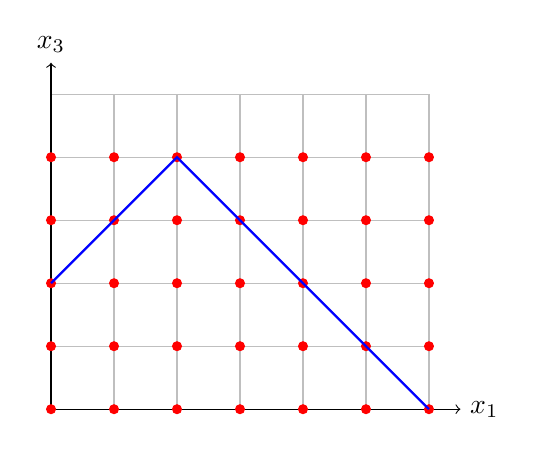
\begin{tikzpicture}[scale=0.8]
    % Grid lines
    \draw[gray!50] (0,0) grid (6,5);
    
    % Axes
    \draw[->] (0,0) -- (6.5,0) node[right] {$x_1$};
    \draw[->] (0,0) -- (0,5.5) node[above] {$x_3$};
    
    % Points
    \foreach \x in {0,...,6} {
        \foreach \y in {0,...,4} {
            \filldraw[red] (\x,\y) circle (2pt);
        }
    }
    
    % Connect points with blue line
    \draw[blue, thick] 
      (0, 2) -- (1, 3) -- (2, 4) -- (3, 3)
      -- (4, 2) -- (5, 1) -- (6, 0);
\end{tikzpicture}

\end{document}